% SIAM Shared Information Template
% This is information that is shared between the main document and any
% supplement. If no supplement is required, then this information can
% be included directly in the main document.
The method stated above was implemented and consolidated into a library called \RACE. The library provides easy interface for parallelizing kernels, user typically just needs to supply the serial code (with dependency) and hardware settings. Library will then parallelize, pin and run the code in parallel. The library is publicly available in the git repository. %TODO

\subsection{Test setup}
In the following we present the performance and convergence results obtained using the library, and compare it against state of art methods. Hardware and matrices as described in \cref{Sec:test_bed} is used for the following benchmarks. As mentioned in \cref{Sec:param_study} parameter $\epsilon_s$ is set to 0.8 and \RCM is used in level construction stage. All the experiments conducted here are using warmed up caches \ie we run the kernel for 100 times initially for warm-up and then we measure performance for the next 500 iteration of the same kernel. Mean performance of this 500 iterations is used to plot the results.

\subsection{Corner Cases}

\begin{figure}[tbhp]
	\centering
	\subfloat[\emph{crankseg\_1}]{\label{fig:crankseg_scaling}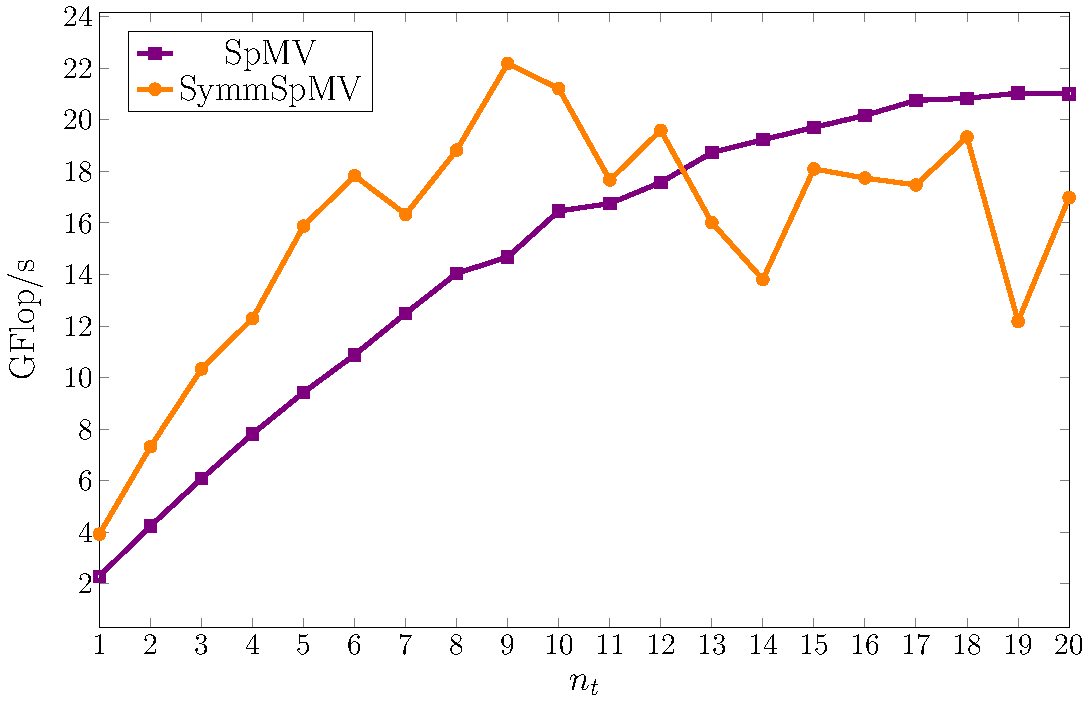
\includegraphics[width=0.45\textwidth , height=0.18\textheight]{pics/results/skx/corner_cases_scaling/crankseg_1}}
	\hspace{1.5em}
	\subfloat[\emph{inline\_1}]{\label{fig:inline_scaling}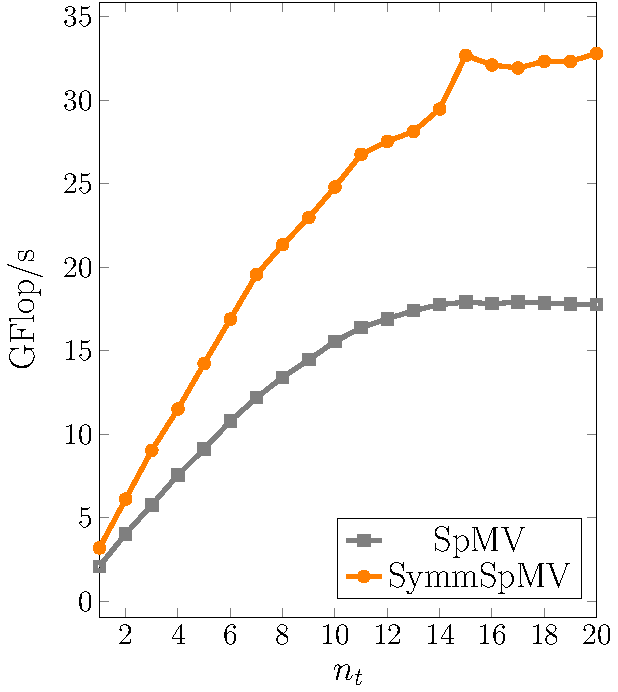
\includegraphics[width=0.45\textwidth , height=0.18\textheight]{pics/results/skx/corner_cases_scaling/inline_1}}	
	\hspace{1.5em}
	\subfloat[\emph{parabolic\_fem}]{\label{fig:parabolic_fem_scaling}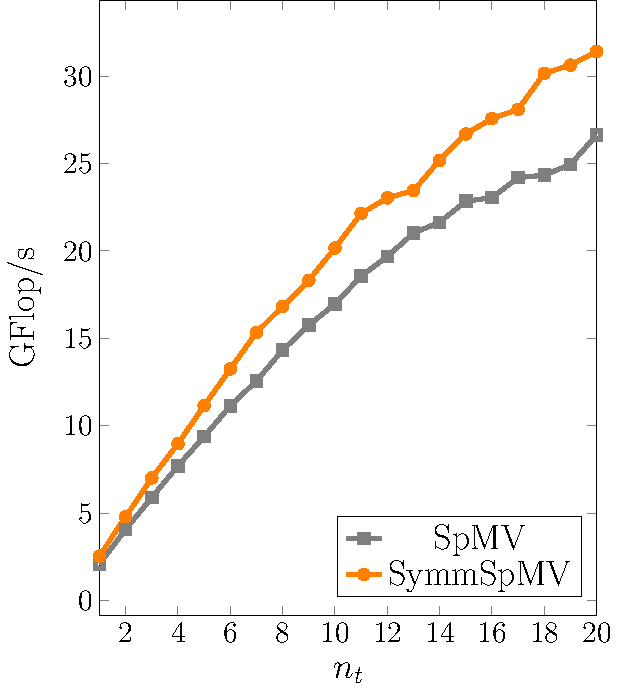
\includegraphics[width=0.45\textwidth , height=0.18\textheight]{pics/results/skx/corner_cases_scaling/parabolic_fem}}
	\hspace{1.5em}
	\subfloat[\emph{Graphene-4096}]{\label{fig:Graphene-4096_scaling} 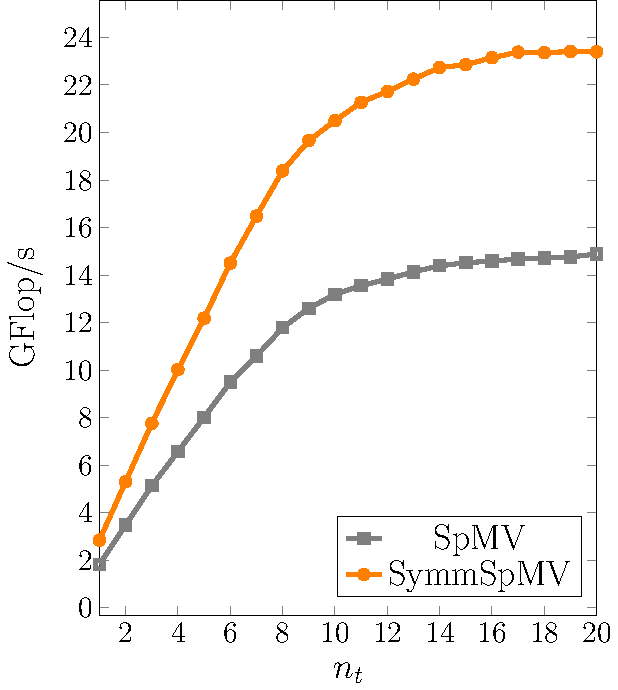
\includegraphics[width=0.45\textwidth , height=0.18\textheight]{pics/results/skx/corner_cases_scaling/Graphene-4096}}	
	\caption{Scaling of \SymmSpmv with RACE compared to \SpMV on one socket of \SKX architecture, for corner case matrices.}
	\label{fig:corner_cases_scaling}
\end{figure}

\Cref{fig:corner_cases_scaling} shows the scaling performance of \SymmSpmv for the corner case matrices on one socket of \SKX architecture. The \emph{crankseg\_1} matrix does not scale well due to it's limited parallelism, as seen in \cref{fig:crankseg_param}, one could further see that the scaling behavior \cref{fig:crankseg_scaling} is exactly in tune with that of the theoretical result seen in \cref{fig:crankseg_param}. Note that due to this bottleneck of parallelism we didn't achieve much benefit from using \SymmSpmv compared to \SpMV.

The \emph{inline\_1} matrix although being third lowest in terms of parallelism in the entire set of test matrices, but it still achieves a high efficiency ($\eta$ = 0.85) for 20 threads (see \cref{fig:inline_param}), leading to good scaling as seen in \cref{fig:inline_scaling}. The saturation in performance after 15 threads is due to the fact that we hit the memory bottleneck, similar behavior can also be observed for \SpMV which is embarrassingly parallel. The saturation occurs at the maximum achievable performance on the given architecture which could easily be verified using the \roofline model (\cite{Williams_roofline}) as shown below:
\begin{align*}
	 P_{max} =&  2 \fracUnit{FMA AVX-512 instruction}{cy*cores}  * 8 \fracUnit{FMA}{FMA AVX-512 instruction} \\
	 & * 2 \fracUnit{Flop}{FMA} * 2.4 \fracUnit{Gcy}{s} * 20 \unit{cores} = 1536  \fracUnit{GFlop}{s} \\	 
	 I_\mathrm{\SpMV} =& \frac{2}{8+4+\frac{8+16}{73}} = 0.162 \fracUnit{Flop}{byte} \text{, assuming best case : $\alpha = \frac{1}{\NNZRmath}$}\\
	 P_\mathrm{\SpMV} =& min(P_{max}, b_s*I_\mathrm{\SpMV})\\
	 P_\mathrm{\SpMV} =& min ( 1536, 0.162*115) = 18.6 \fracUnit{GFlop}{s}
\end{align*}

As seen we achieve 17.8 GFlop/s which is close to the theoretical maximum of 18.6 GFlop/s for \SpMV. Similar derivation can be done for \SymmSpmv and one could see $P_\mathrm{\SymmSpmv}$= 34.5 GFlop/s, which is approximately twice that of \SpMV since $I_\mathrm{\SymmSpmv}$ is almost a factor two higher than $I_\mathrm{\SpMV}$ for matrix with moderate \NNZR. From \cref{fig:inline_scaling} one can observe that at saturation we reach close to theoretical values. The cushioning effect of memory bandwidth bottleneck is also evident from \cref{fig:inline_scaling}, where we see that due to this saturation decrease in $\eta$ to a certain extent would not effect the socket level performance, it would just shift the knee of saturation towards right.

In the case of \emph{parabolic\_fem} matrix we theoretically have a good efficiency as seen from \cref{fig:parabolic_fem_param}, but here we do not see any saturation in performance (see \cref{fig:parabolic_fem_scaling}), even \SpMV does not have this saturation behavior. If one calculates the maximum  theoretical performance by \roofline model as shown in previous example one would see that $P_\mathrm{\SpMV}$=15 GFlop/s and $P_\mathrm{\SymmSpmv}$=19 GFlop/s, but we achieve more than these values 26.5 and 31.5 GFlop/s respectively, this is because the matrix is small enough ($\approx$ 46 MB for full matrix and $\approx$ 23 MB for symmetric storage) and it just fits in caches (combined L2 and L3) of the \SKX architecture. Since the caches scales well on this architecture we don't observe the saturation behavior. Also observe that difference between \SymmSpmv and \SpMV is not two times here since non-zeros per row is small (\NNZR=7, \NNZRSYMM=4). 

\emph{Graphene-4096} matrix on the other hand is a matrix with efficiency similar to \emph{parabolic\_fem} but with much larger size ($\approx 2 GB$) resulting in matrix data always coming from main memory. This therefore shows dominant saturation behavior and since we achieve good efficiency ($\eta$) the knee of saturation begins at a well early stage for \SymmSpmv compared to  the case of \emph{inline\_1} where the efficiency was lower in comparison resulting in smaller \threadEff.

\begin{comment}


\begin{figure}[thbp]
  	\centering
   	\subfloat[RACE performance compared to SpMV]{\label{fig:race_ivy}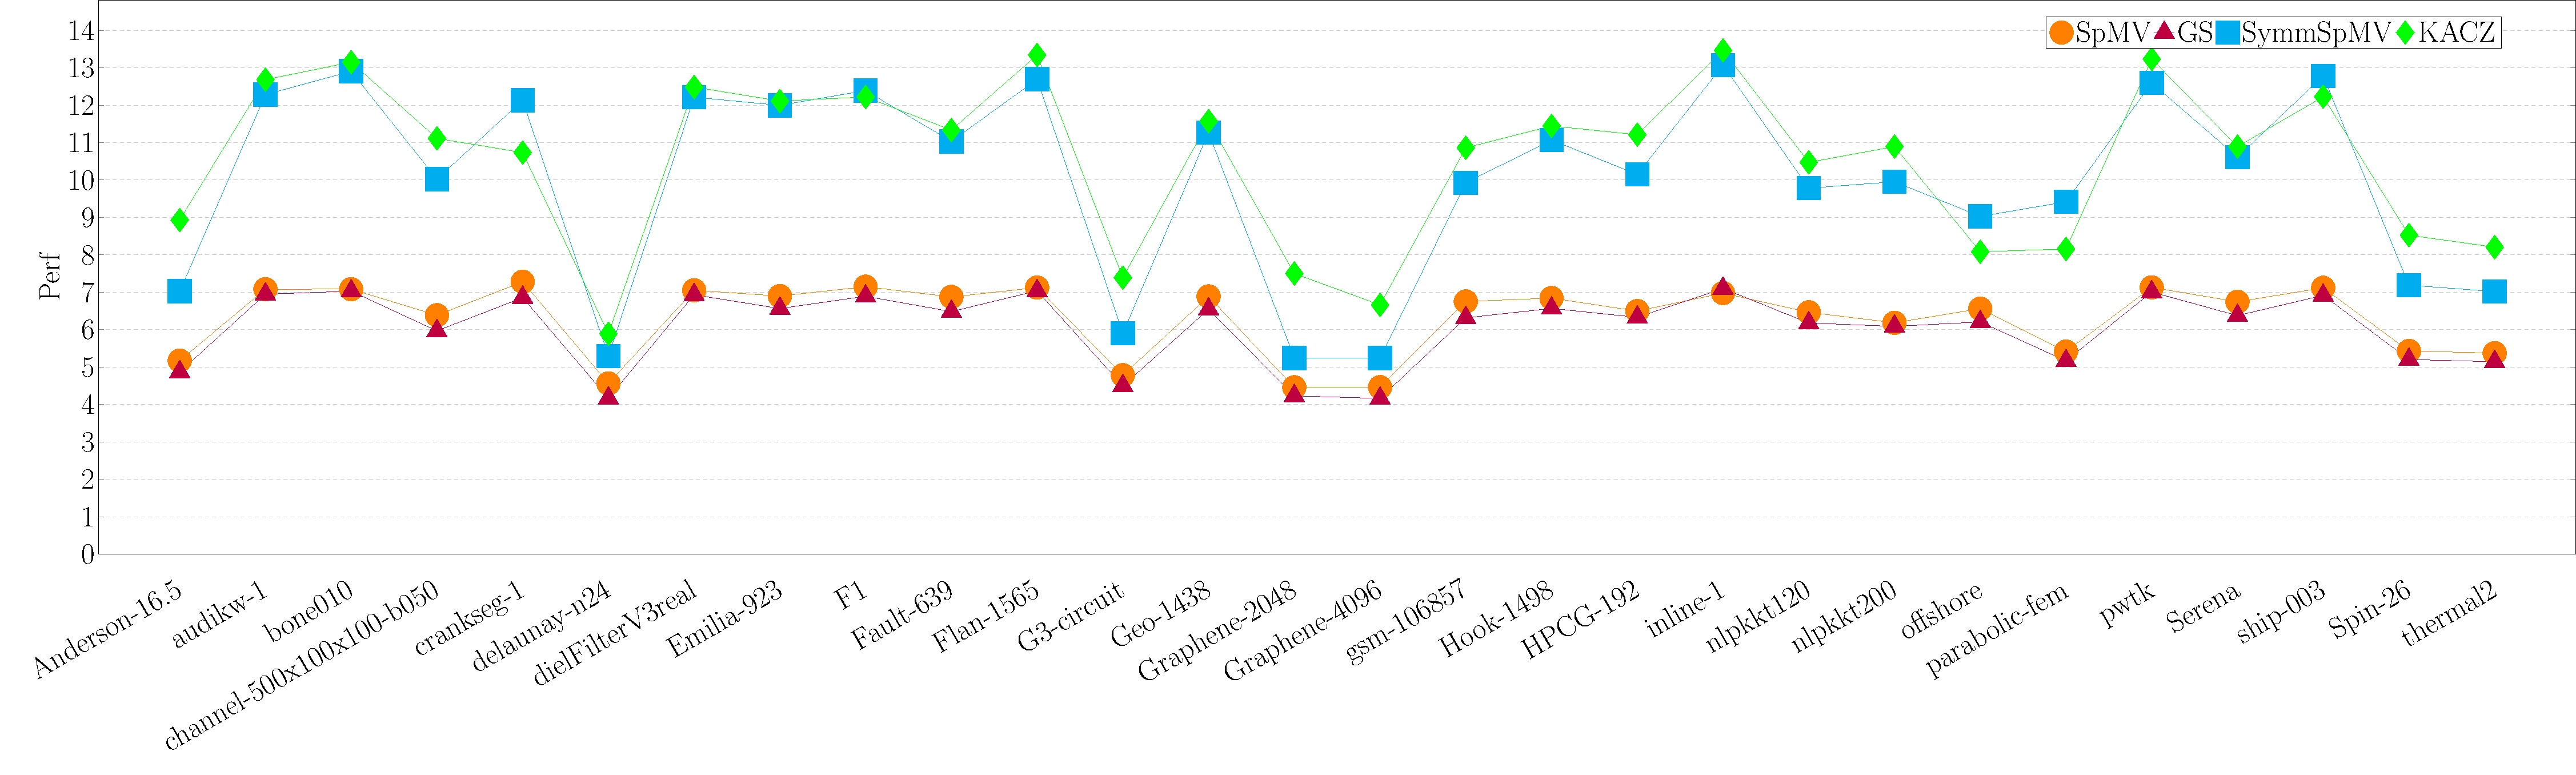
\includegraphics[width=0.49\textwidth, height=0.11\textheight]{pics/results/ivy/race}}
    \subfloat[SymmSpMV Comparison]{\label{fig:symm_spmv_ivy}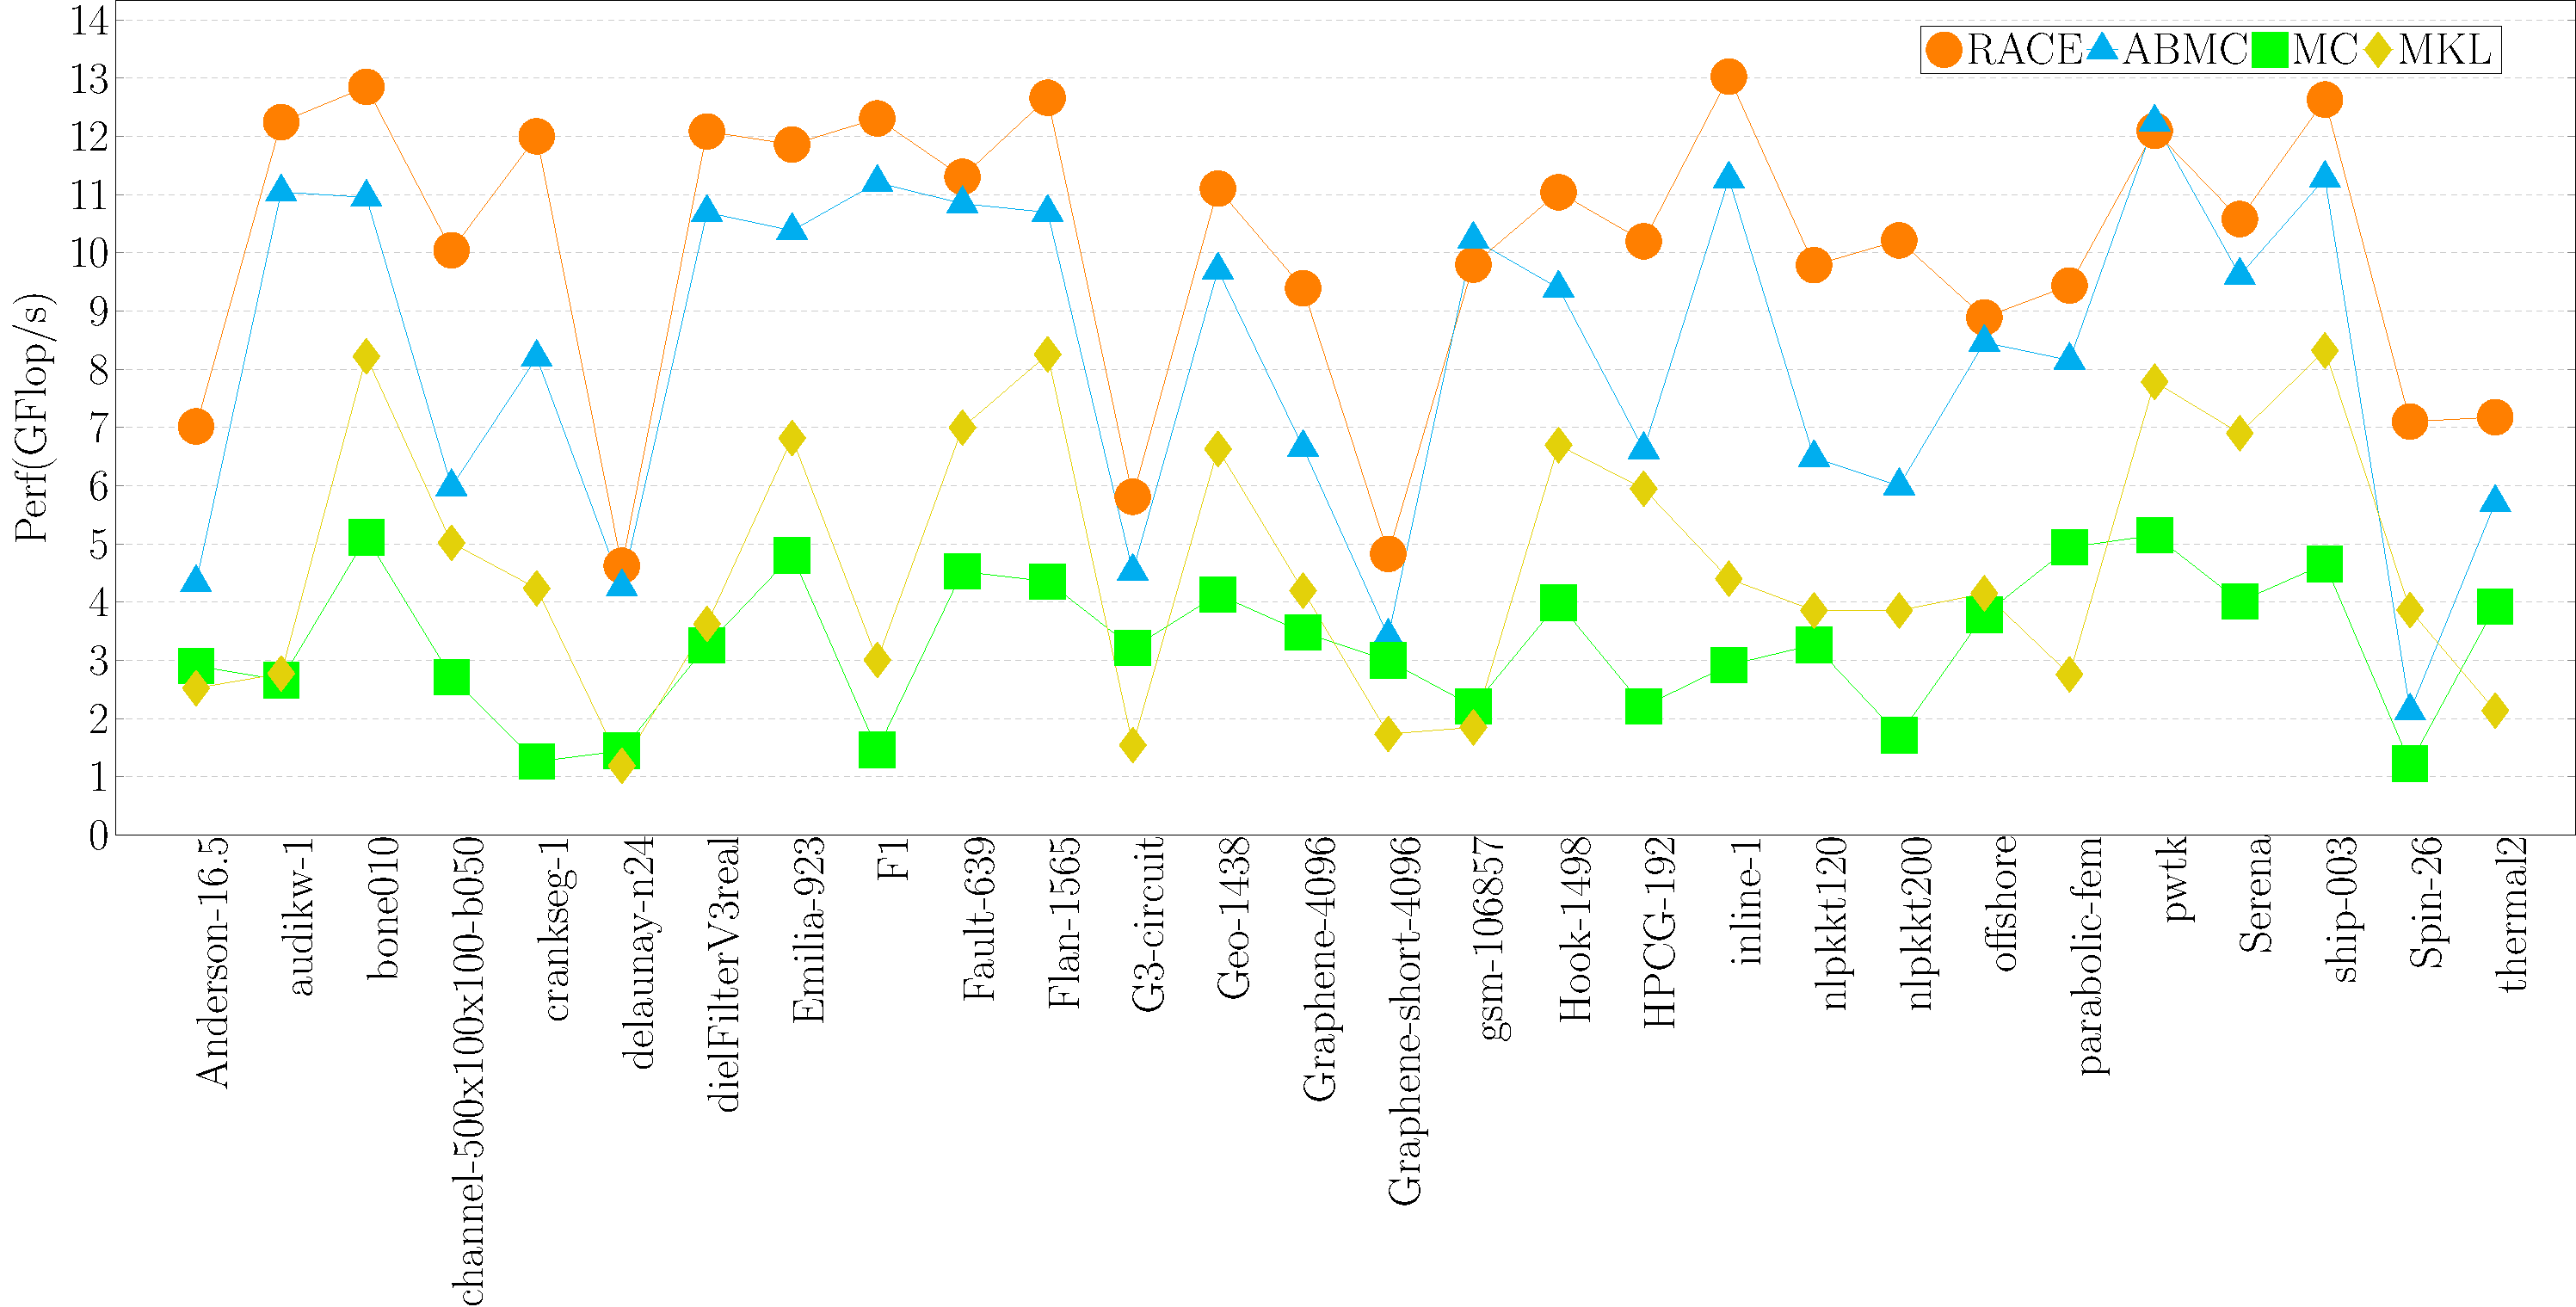
\includegraphics[width=0.49\textwidth, height=0.11\textheight]{pics/results/ivy/symm_spmv}}
    \hspace{1em}
    \subfloat[GS Comparison]{\label{fig:gs_ivy}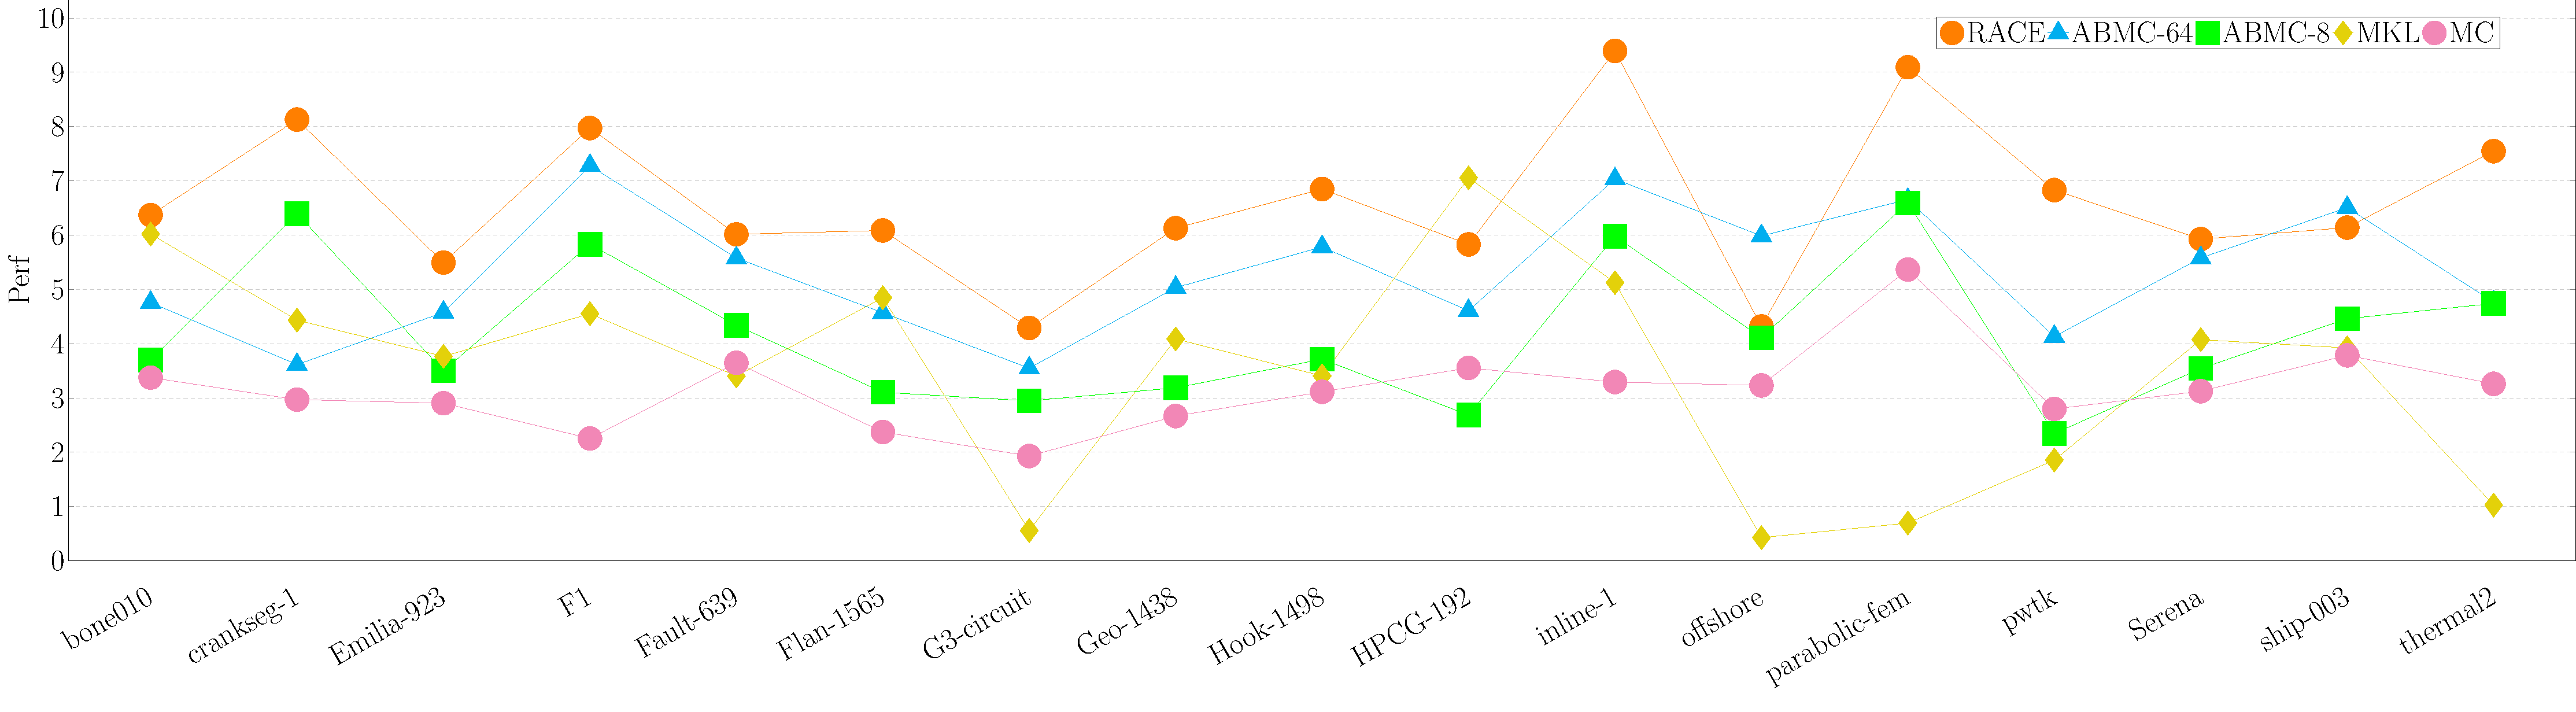
\includegraphics[width=0.49\textwidth, height=0.11\textheight]{pics/results/ivy/gs}}
    \subfloat[KACZ Comparison]{\label{fig:kacz_ivy}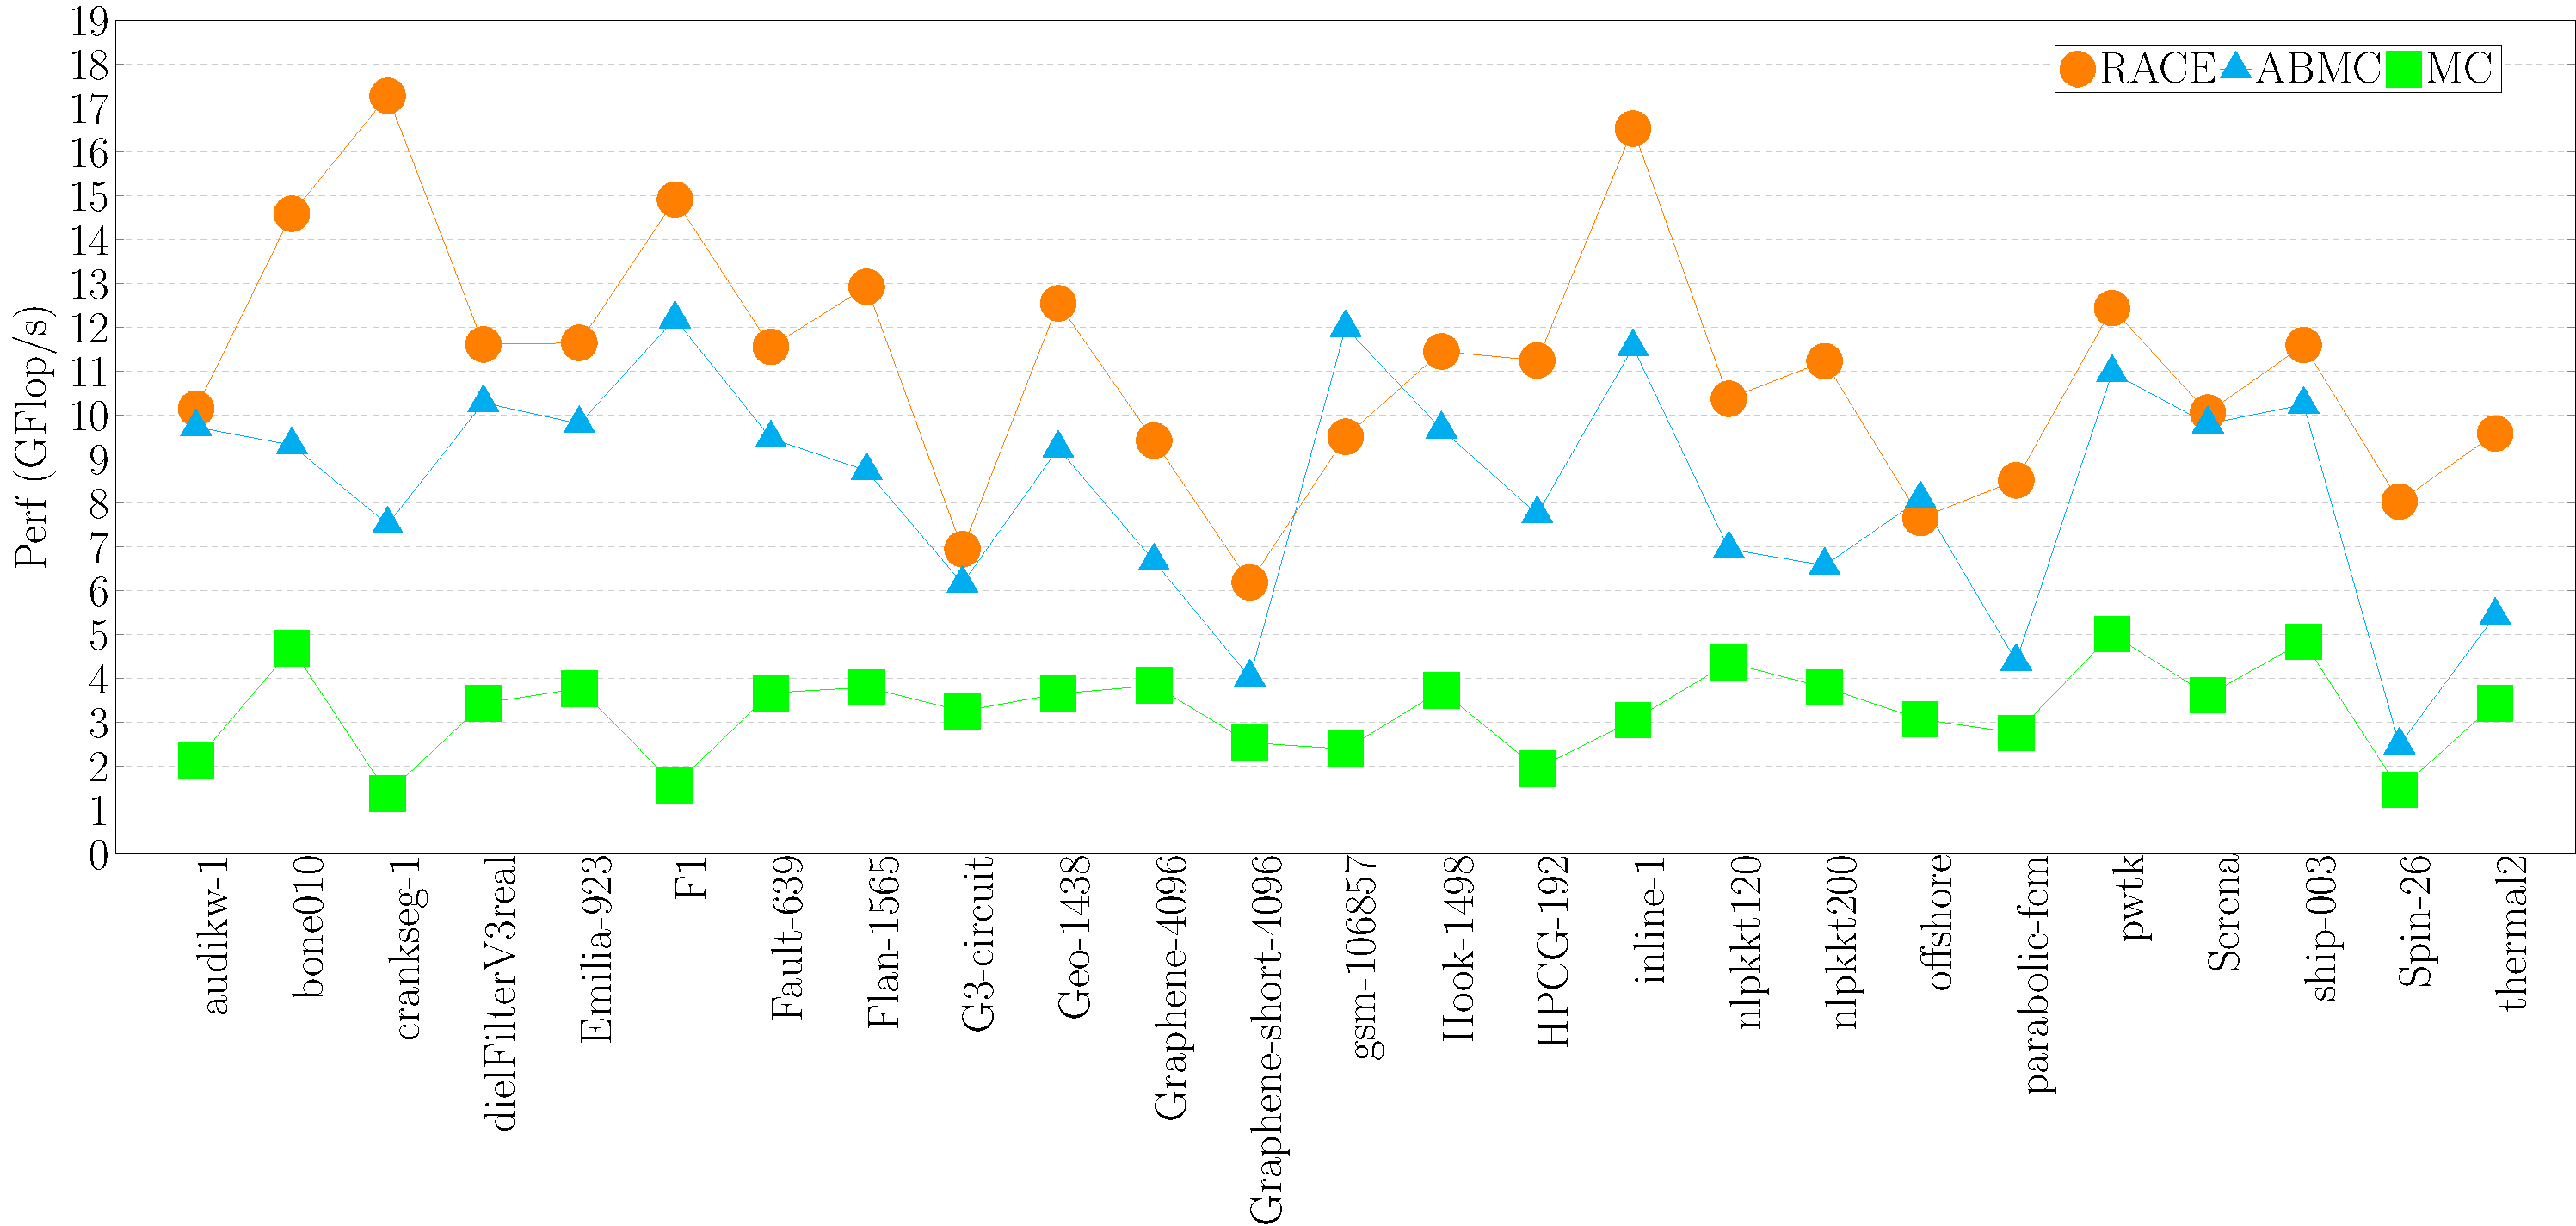
\includegraphics[width=0.49\textwidth, height=0.11\textheight]{pics/results/ivy/kacz}}
    \caption{Performance results on \IVB}
    \label{fig:ivy}
\end{figure}


\begin{figure}[thbp]
	\centering
	\subfloat[RACE performance compared to SpMV]{\label{fig:race_skx}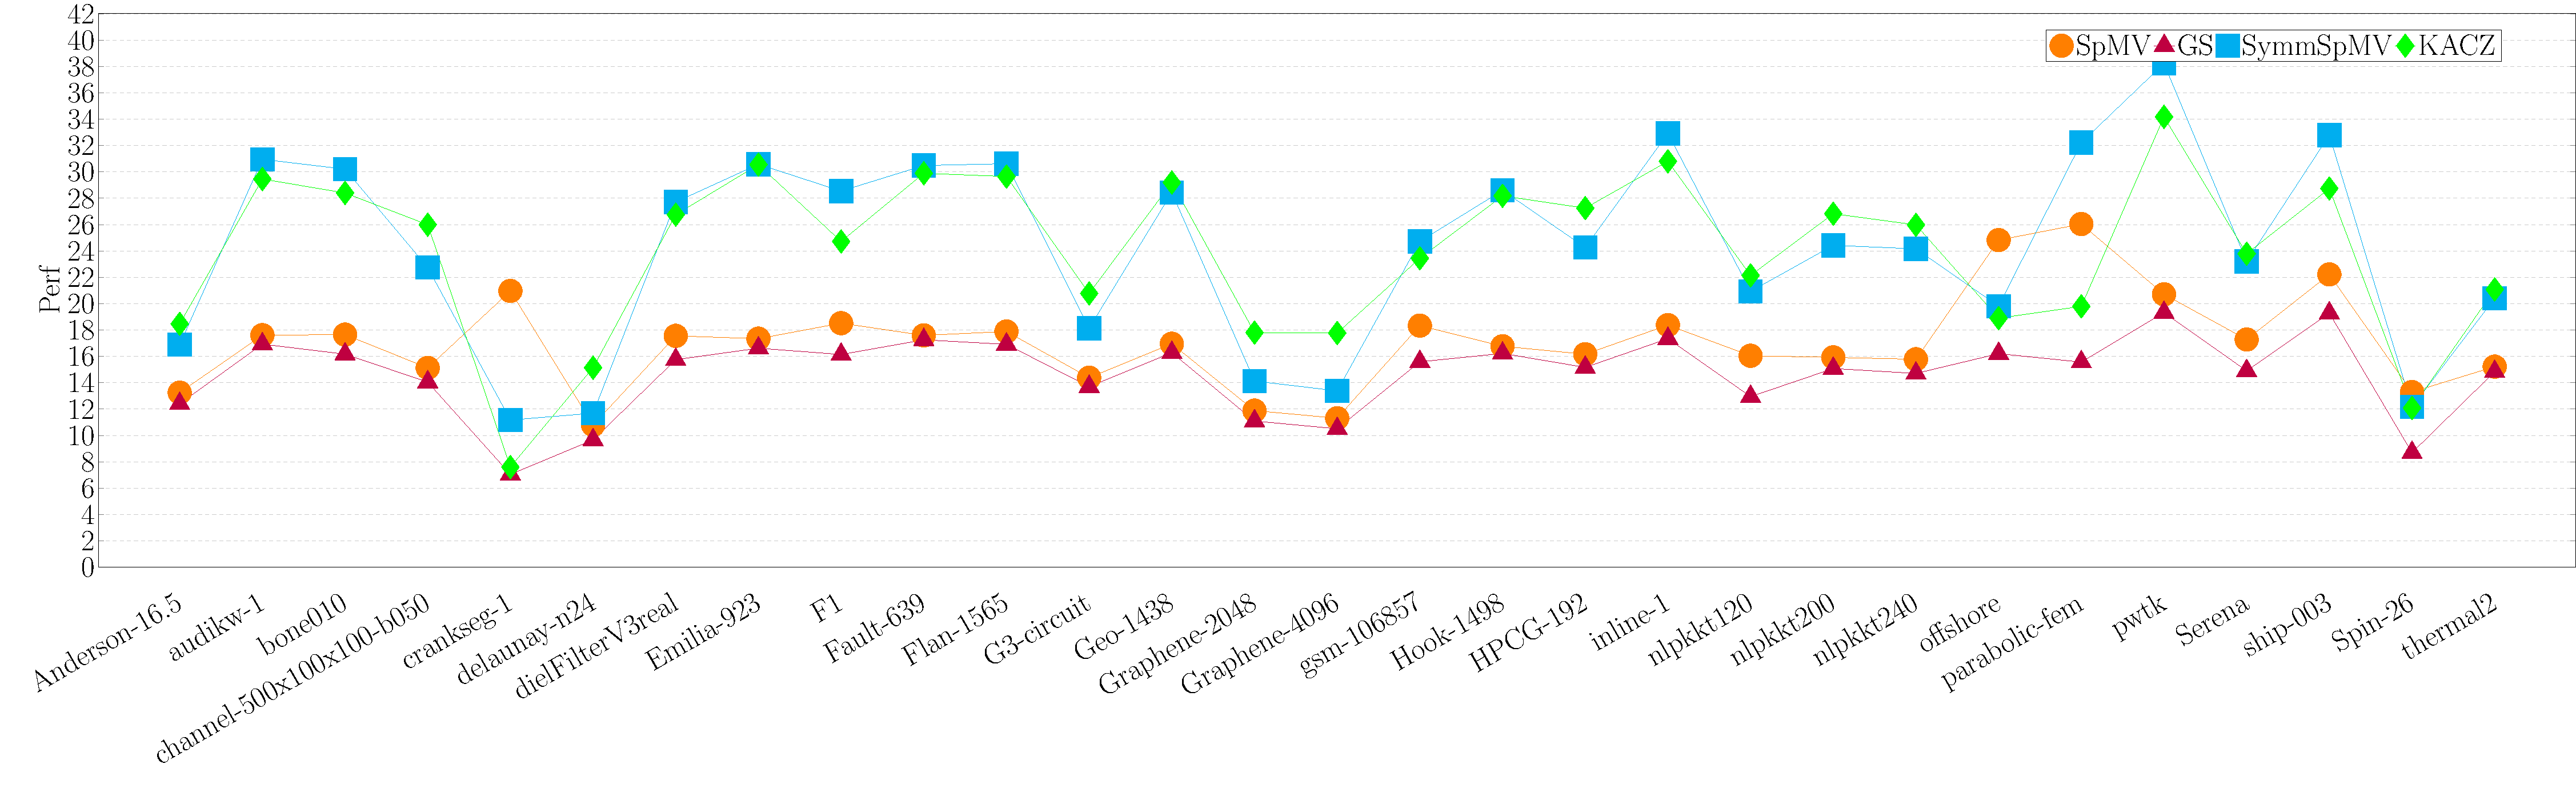
\includegraphics[width=0.49\textwidth, height=0.11\textheight]{pics/results/skx/race}}
	\subfloat[SymmSpMV Comparison]{\label{fig:symm_spmv_skx}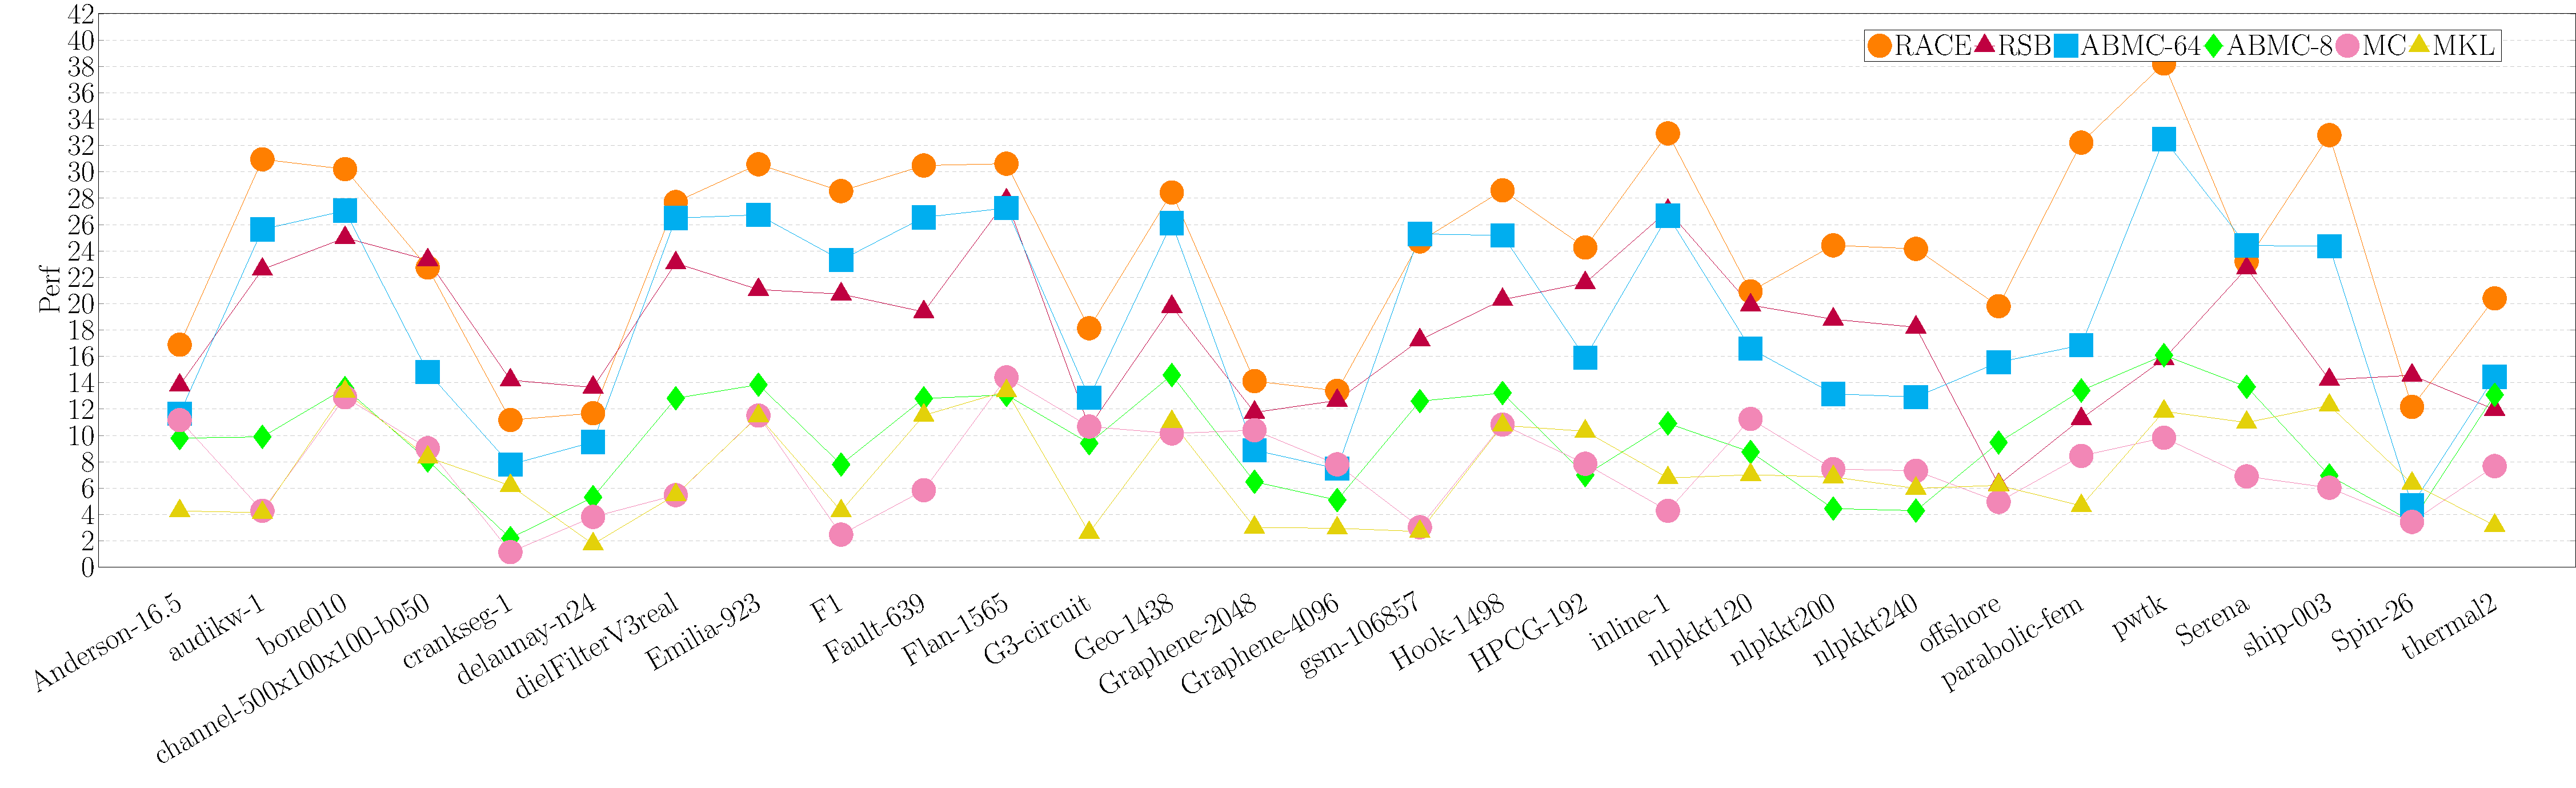
\includegraphics[width=0.49\textwidth, height=0.11\textheight]{pics/results/skx/symm_spmv}}
	\hspace{1em}
	\subfloat[GS Comparison]{\label{fig:gs_skx}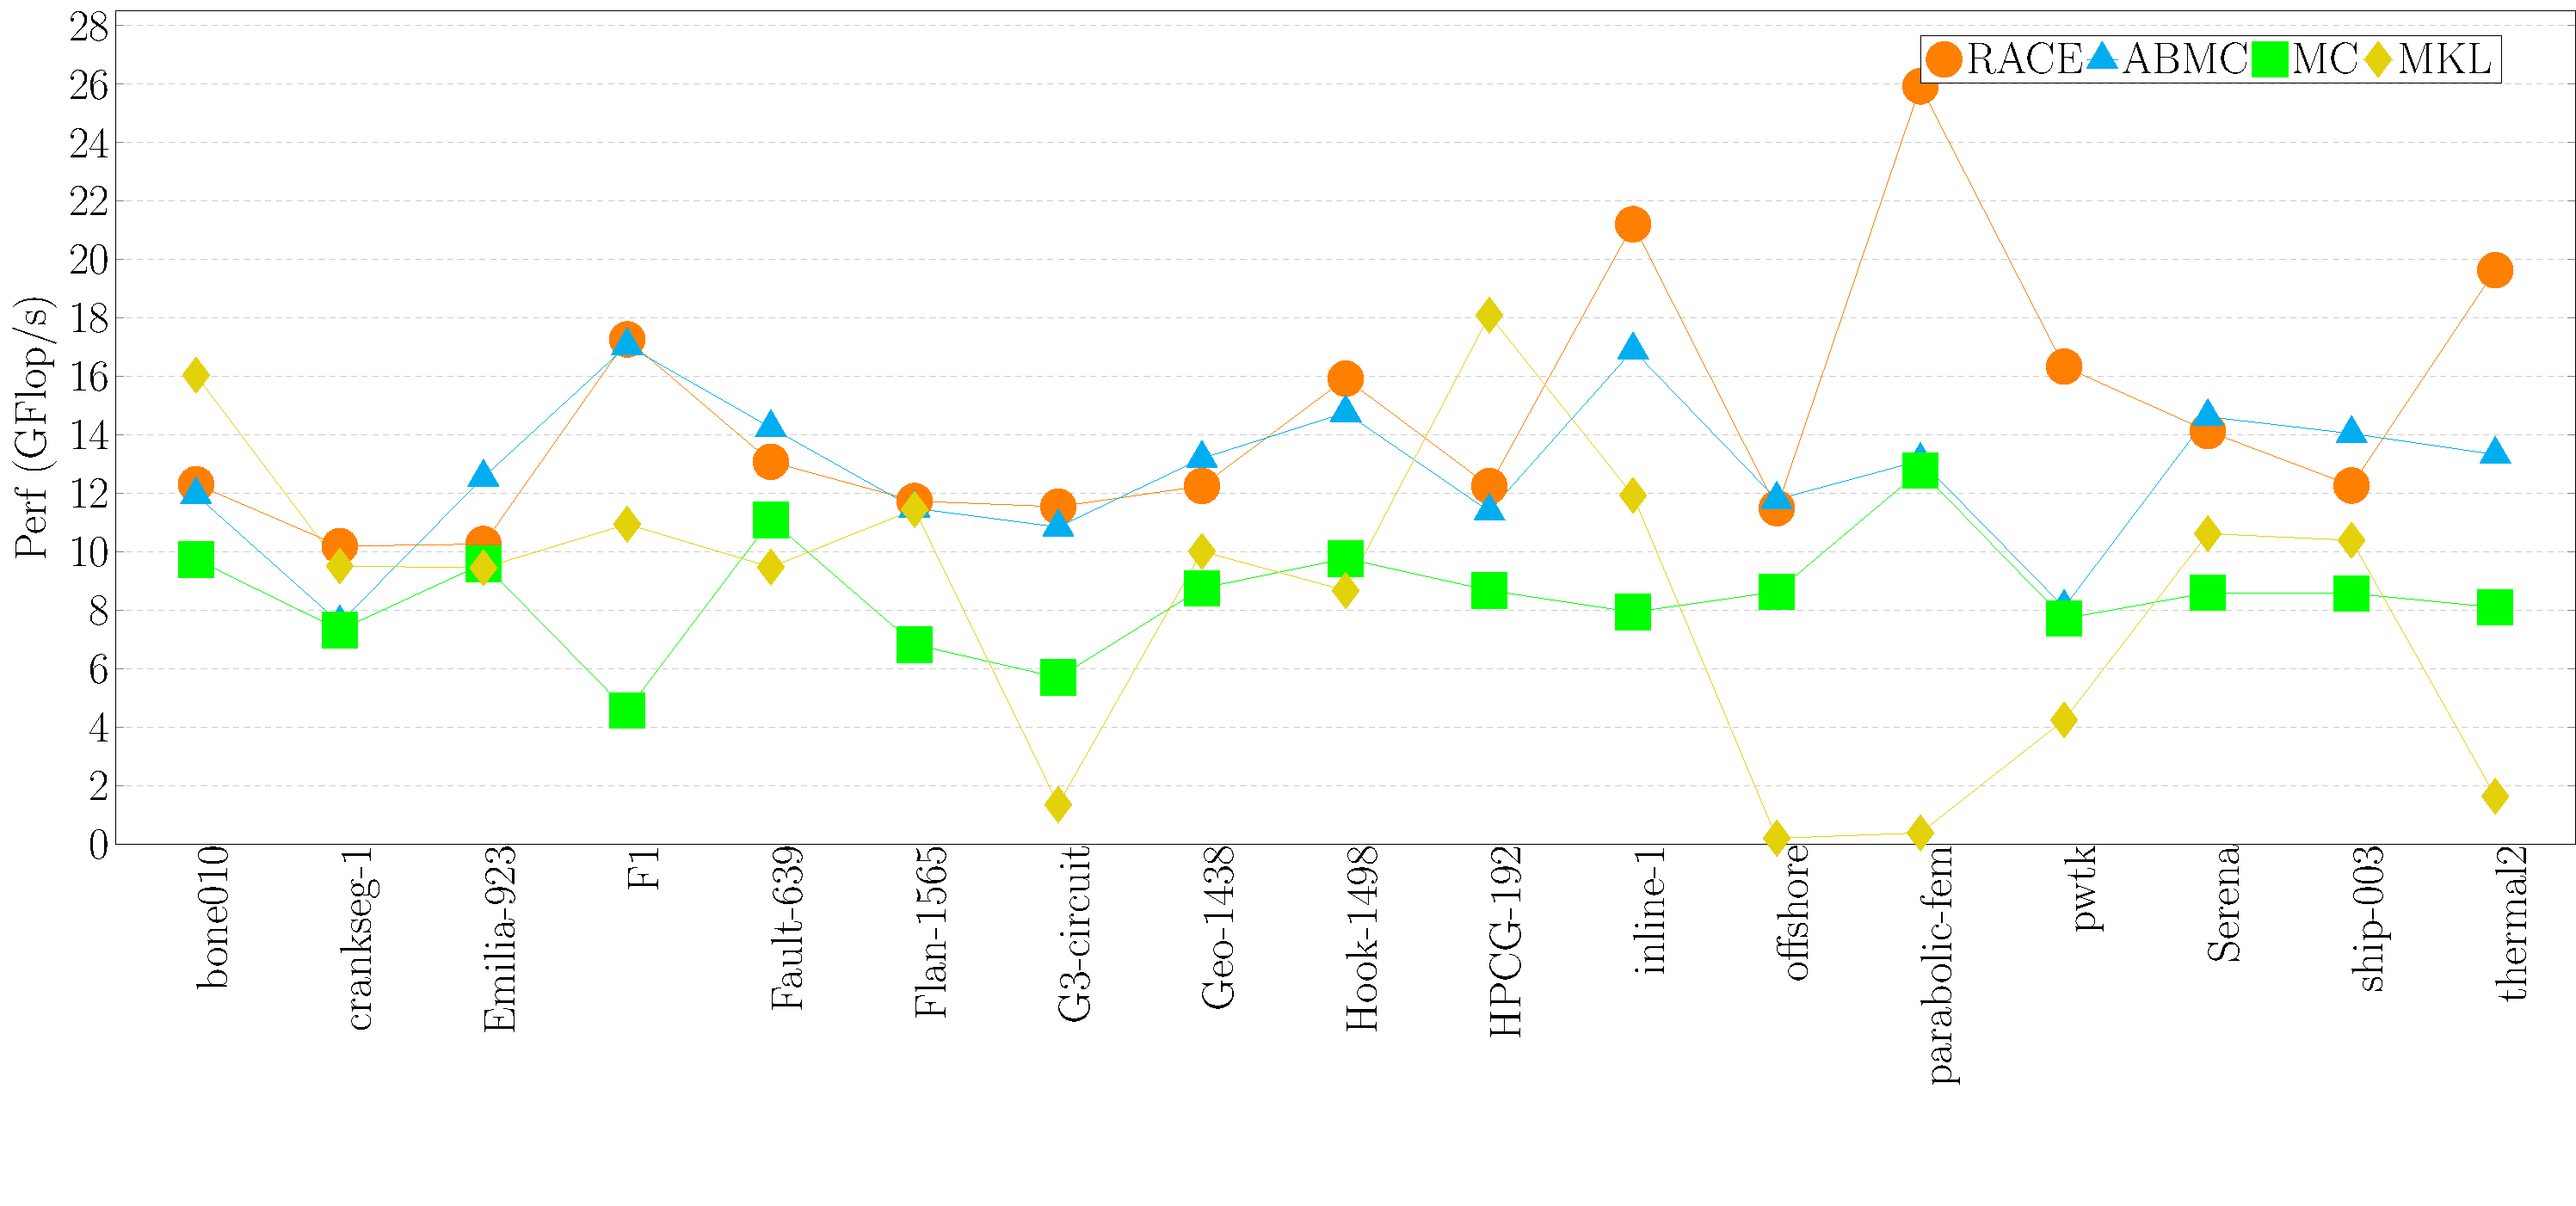
\includegraphics[width=0.49\textwidth, height=0.11\textheight]{pics/results/skx/gs}}
	\subfloat[KACZ Comparison]{\label{fig:kacz_skx}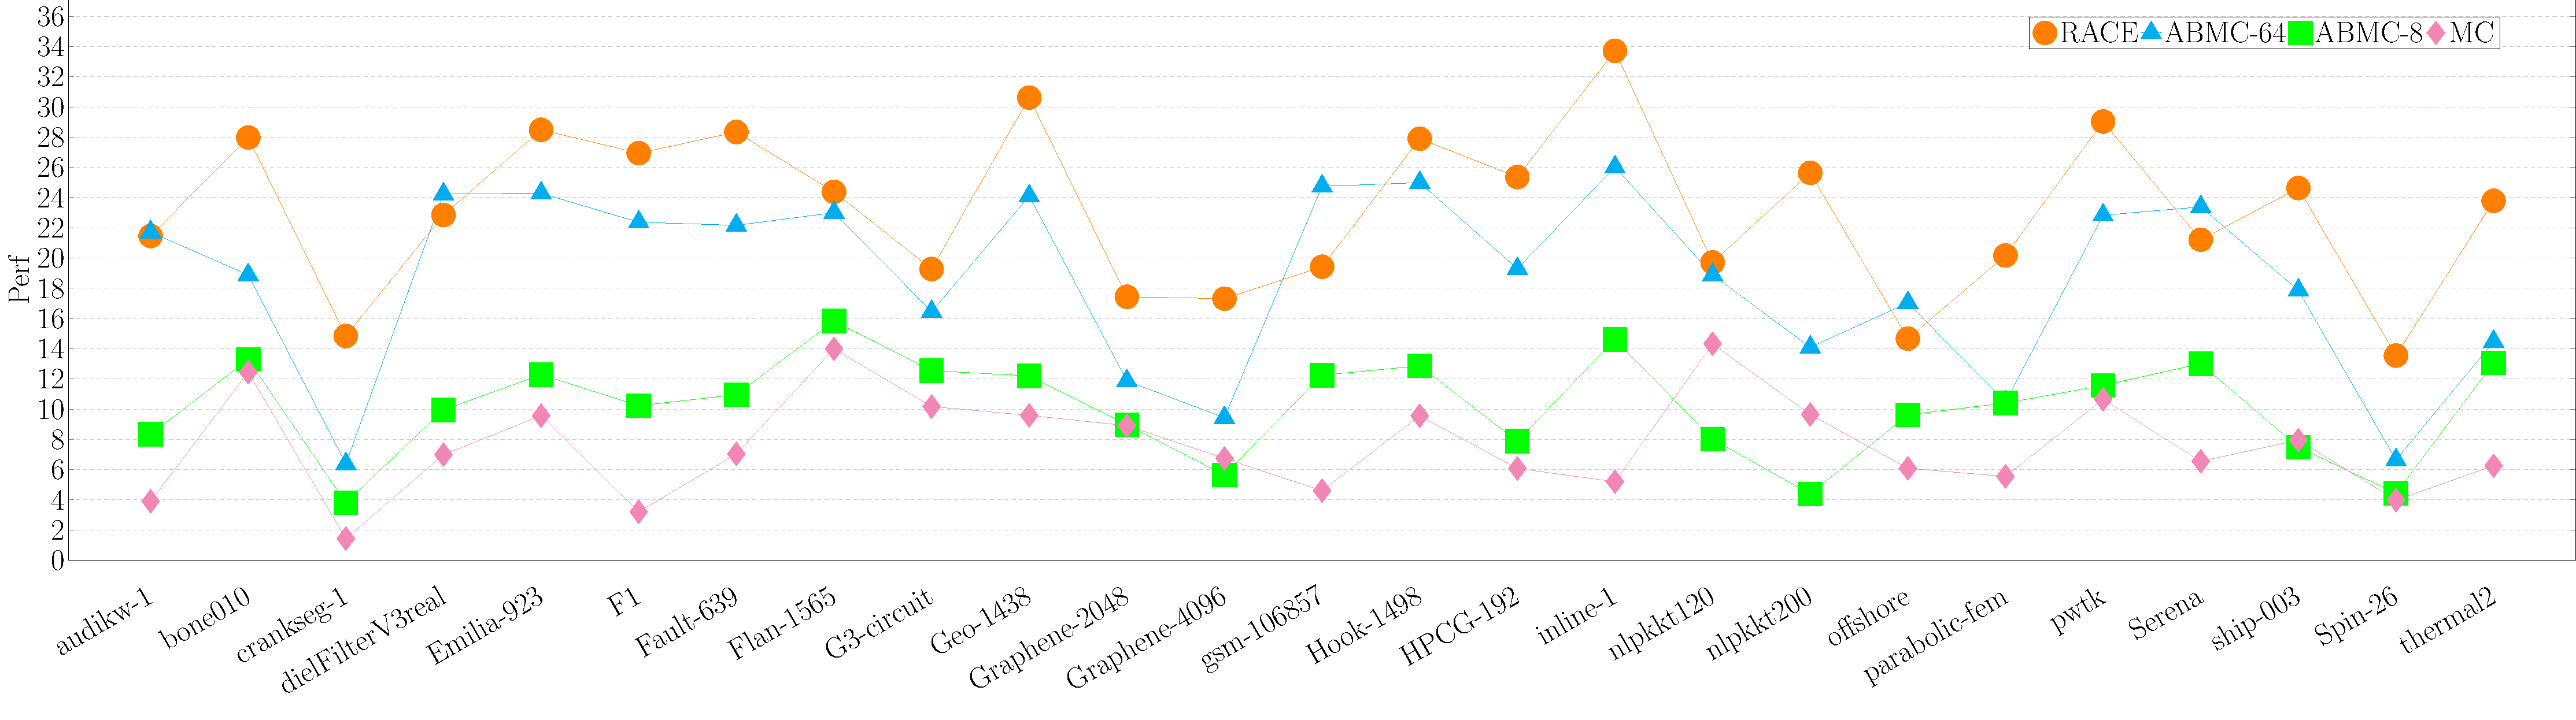
\includegraphics[width=0.49\textwidth, height=0.11\textheight]{pics/results/skx/kacz}}
	\caption{Performance results on \SKX}
	\label{fig:skx}
\end{figure}

\subsection{Main points to discuss}
\begin{itemize}
	\item Mention about specific setups like RCM for MKL and RSB, using IE for MKL
	\item Relate roofline model and the performance graphs of RACE compared to SpMV. 
	\item Point out on \IVB we reach close to ideal performance in every case, and on \SKX except for corner cases like crankseg and offshore we reach close to ideal performance. The drop in corner cases like crankseg and offshore on \SKX is due to lack of parallelism attained by RACE and associated load imbalances. This effect shows up on \SKX rather than \IVB since \SKX has 20 threads compared to 10 on \IVB.
	\item Point out that for cases like Graphene, Spin, parabolic\_fem we don't see 2 fold increase in GFlop/s for KACZ, and SymmSpMV. This is due to the fact here \NNZR is very small like 4, 14 and 7 which causes two problems. For KACZ kernel there is one division per row and this causes a performance drop as evident in Spin matrices, also this effect can be observed for GS kernel. For SymmSpMV kernel the \NNZR decreases almost by half since we operate only on upper triangular part and with short loop over \NNZR no effective vectorization and modulo unrolling can be done.
	\item Matrices like crankseg-1, and offshore are also really small making some part of data fit in cache, this is the reason why they achieve performance above RLM.
	\item Discuss why we chose the methods for comparison. MC and ABMC are common in literature for \DONE coloring, MKL methods are standard library used in many productive codes, also it uses level-scheduling (not explicitly stated but we believe) for kernels like GS and enables us to compare with methods that do not disturb convergence. RSB enables to compare with methods using different data format and it has been shown this method has an upper hand in this category. 
	\item Comparison with SymmSpMV shows the behavior of different methods for \DTWO coloring. Here we see in almost all of the case RACE and RSB has an upper hand on \IVB, although in some cases like offshore RACE clearly has an advantage. ABMC methods follow these methods. MKL and MC does not deliver good performance. For \SKX architecture \RSB falls behind \ABMC, we thing this is because of the requirement of \RSB to lock rows and cols of the submatrix on which a thread is working, becoming a bottleneck at high thread counts.
%	\item Explain SKX has slower stores, observable from load:copy benchmark ratio leading to SymmSpMV and KACZ not achieving two times SpMV, but on BDW this ratio is not much. This will get interesting with \EPY.
	\item Maybe tell RSB and 16-bit integer.
	\item Discuss with methods like ABMC and MC the performance especially drops for large matrices like Graphene, Spin, nlpkkt due to worsening of data locality ($\alpha$). Show sparsity pattern and \LIKWID meaurements. 
	\item Tell GS and KACZ performance includes also takes iterations into consideration (as shown in paper). Tell we do only a \DONE coloring for GS and \DTWO for KACZ. We use only matrices where GS can be applied and similarly for KACZ. Also we just compare against readily available solutions. Therefore RSB is left out for GS and RSB and MKL left out for KACZ.
	
\begin{figure}[thbp]
	\centering
	\subfloat[\SYMMGS iterations required by different methods compared to exact MKL kernel] {\label{fig:iter_gs}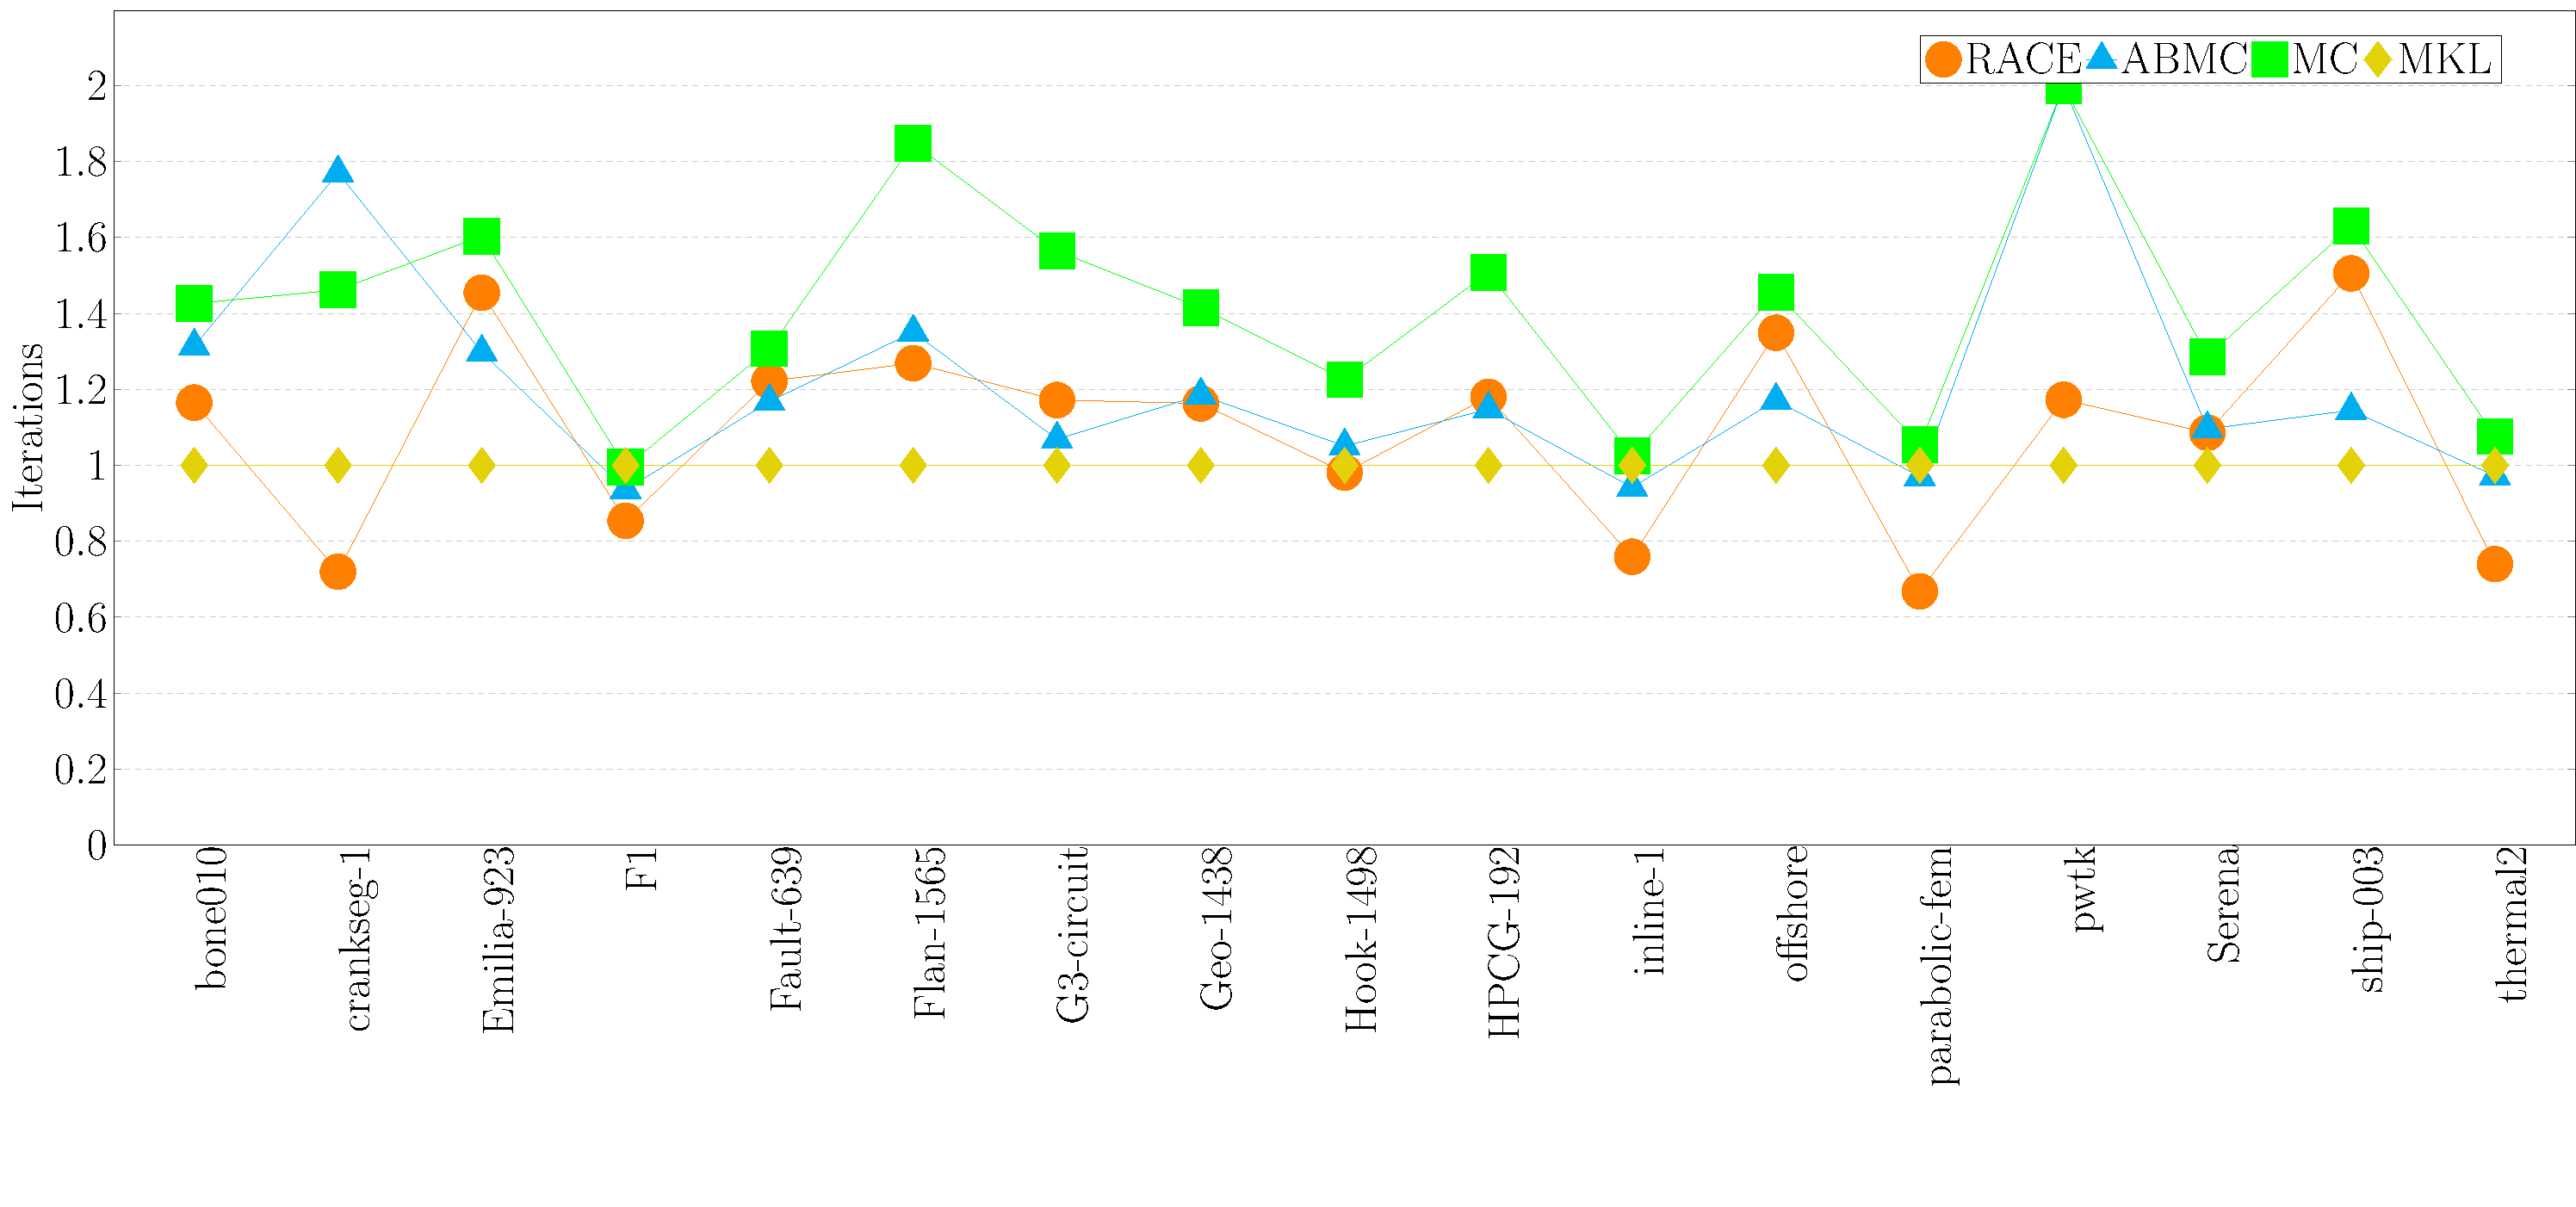
\includegraphics[width=0.49\textwidth, height=0.11\textheight]{pics/results/skx/iter/gs/plot}}
	\subfloat[\SYMMKACZ iterations required by different methods compared to exact Serial kernel] {\label{fig:iter_kacz}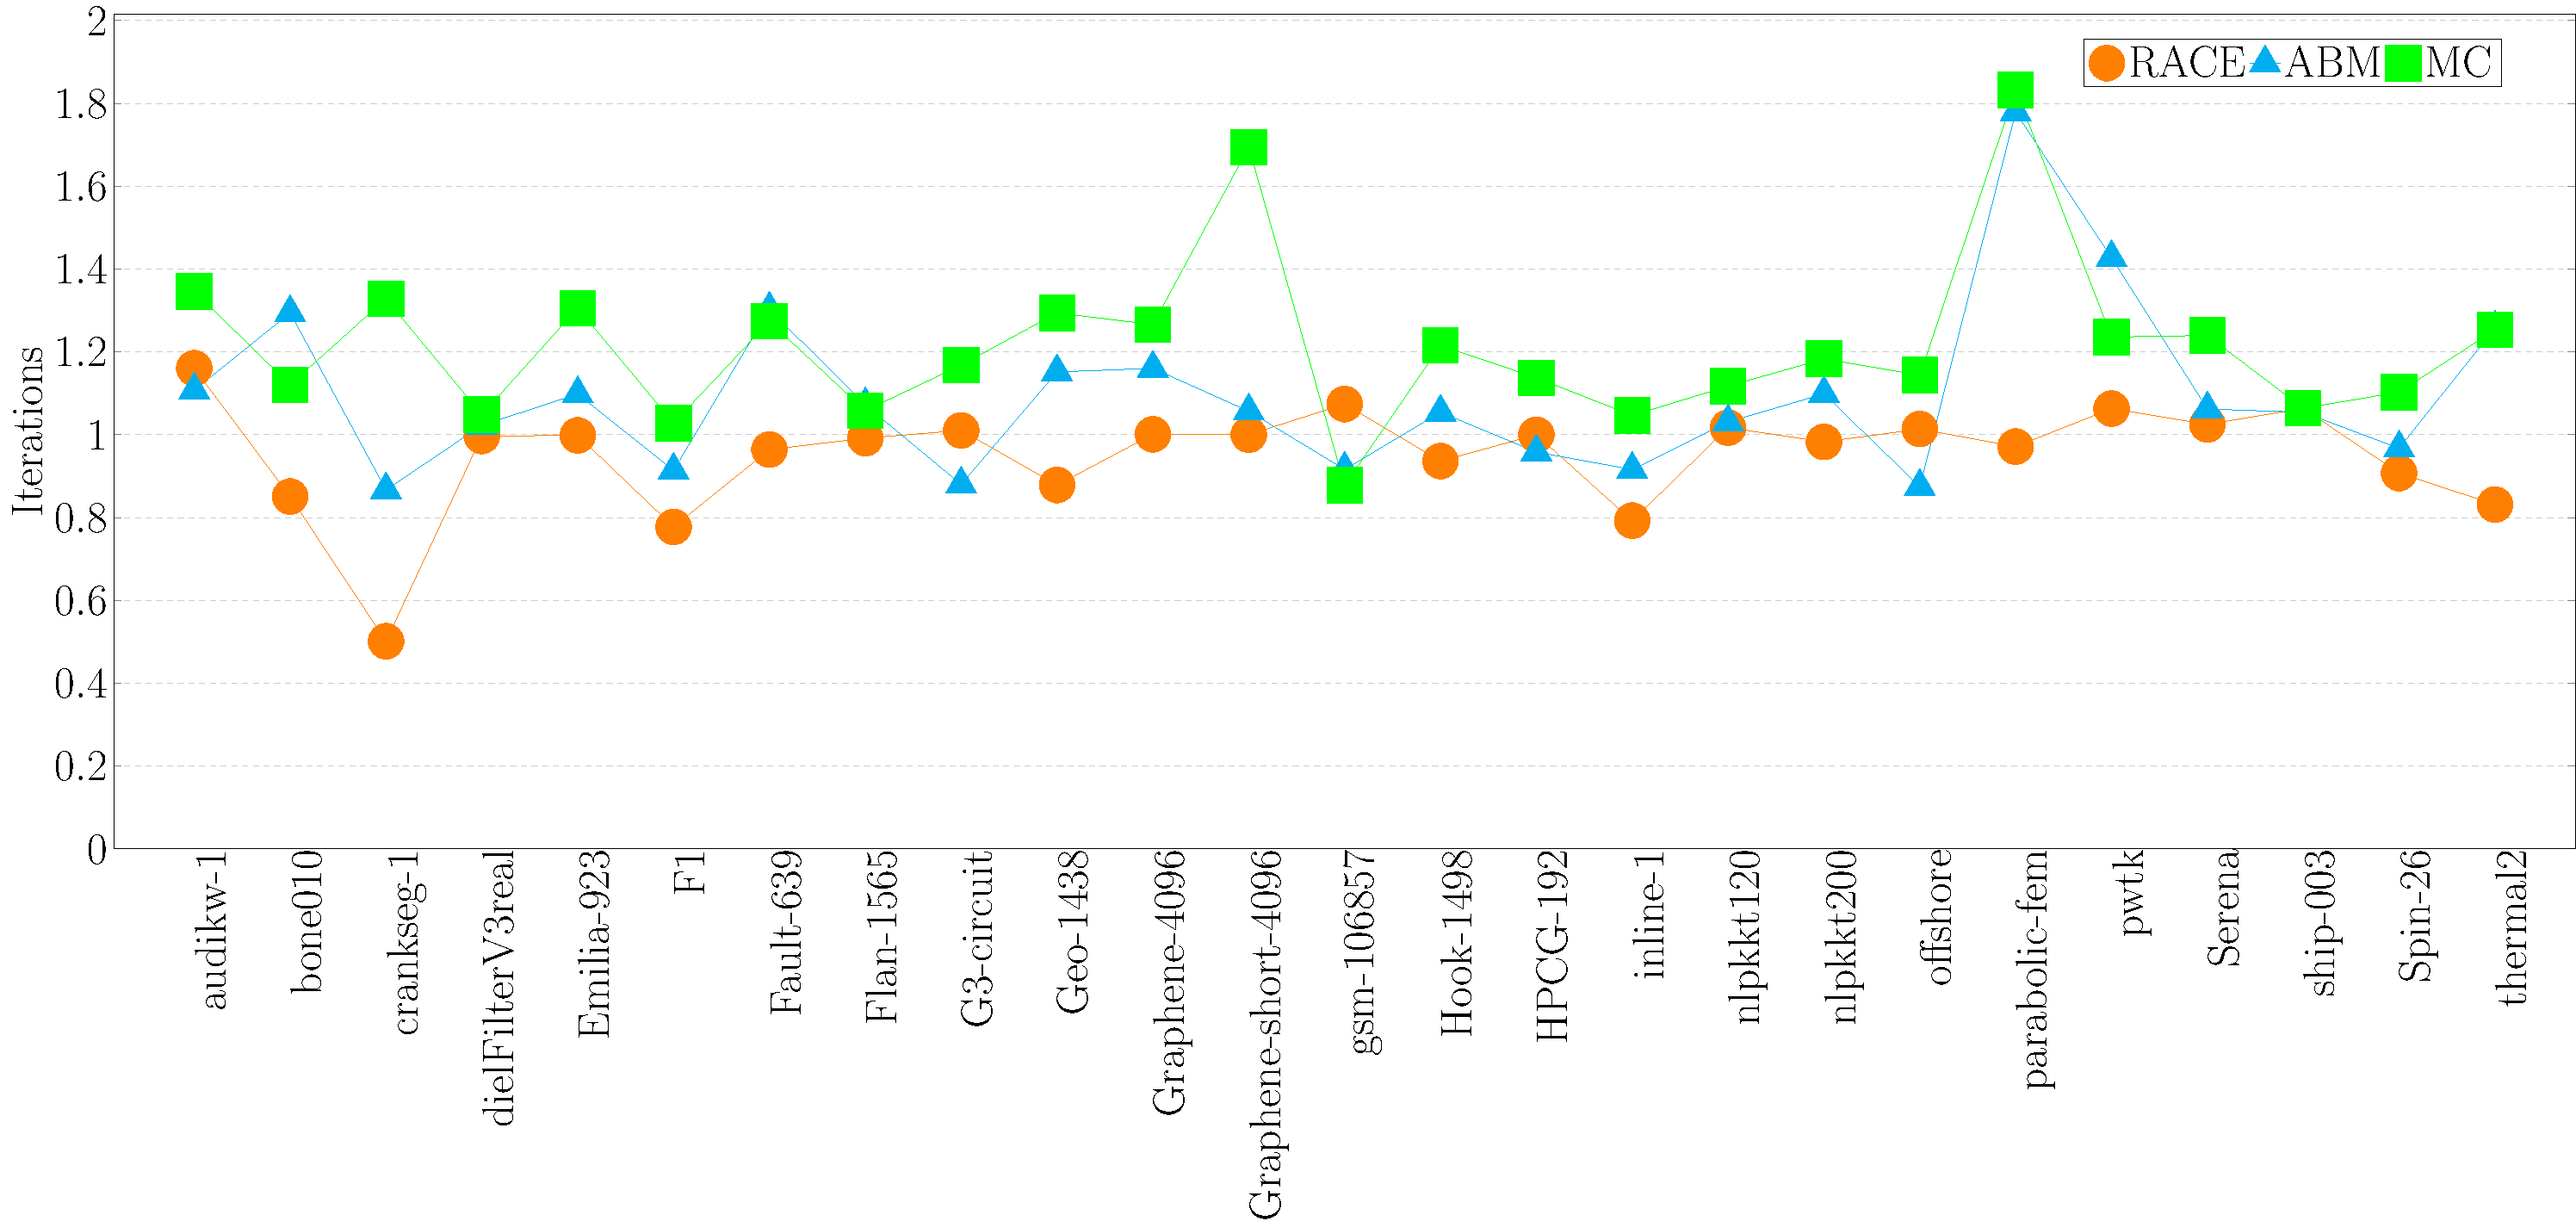
\includegraphics[width=0.49\textwidth, height=0.11\textheight]{pics/results/skx/iter/kacz/plot}}
	\caption{Convergence behavior of \SYMMGS and \SYMMKACZ at 20 threads}
	\label{fig:conv_behavior}
\end{figure}
	
	\item For GS RACE has an upper hand on \IVB and on \SKX RACE and ABMC have almost similar performance on \SKX, although for some cases RACE has huge advantage. Reason for this advantage is due to slight decrease in iterations for RACE (see \cref{fig:iter_gs}) and slight improvement in performance compared to ABMC for \DONE case. For offshore case RACE performs worser that ABMC, this is because here with RACE one requires more iterations. Also note that all the large matrices which we had are unsuitable for GS sweep as they do not converge, but for large matrices the performance drops again for ABMC method due to degrading of $\alpha$ factor. (Maybe just put perf. pictures).
	\item Main advantage of RACE method comes with kernels having \DTWO dependencies like SymmSpMV and KACZ since here methods like ABMC require more colors and their locality degrades further since here within a color rows have to be structurally orthogonal (rows shouldn't have common column entries). Performance on KACZ shows this advantage. Here we again see for moderately large matrices the advantage is higher. Iteration behavior between methods remains similar to GS (see \cref{fig:iter_kacz}).
\end{itemize}
 
\end{comment}
